\chapter{Pruebas}\label{chap:Pruebas}
En el penúltimo capítulo del documento se mostrarán los resultados del proyecto; se hará un análisis de la ejecución juego (su ) y del rendimiento del simulador sobre el que se ejecuta.

\section{Descripción de las pruebas}
\subsection{Escenarios}
En estas secciones se verifica el funcionaiento y se analiza el rendimiento de todo aquello que vimos en el capítulo \ref{chap:Integration}. Hemos decidido llevar a cabo las pruebas en dos entornos diferentes, para ponderar ventajas e inconvenientes de cada uno de ellos. Estos se describen a continuación:
\begin{itemize}
\item \textbf{caso 1: GNS3 nativo}. Se trata del escenario sobre el que todo el desarrollo del proyecto ha sido ejecutado. El entorno consiste en una máquina física con Windows 10 desde donde el juego es ejecutado y GNS3 debe estar corriendo. Como se trata de un sistema operativo Windows, nodos como los de OpenWRT necesitan ser montados sobre un GNS3 VM, lo cual implica hacer uso de un hipervisor (aquí usaremos Virtualbox, pues aunque su rendimiento es inferior al de VMware, es open source) donde instalarlo. El proceso de despliegue es entonces algo tedioso, ya que requiere de una instalación de GNS3, una configuración apropiada del mismo y una máquina virtual con GNS3 VM.

Como se ejecuta sobre la máquina física, cuenta con todas las prestaciones que listamos en la sección \ref{sec:hardware}.
\item \textbf{Caso 2: GNS3 en una máquina virtual}. Este caso pretende acabar con ese proceso. La idea aquí es usar una sola máquina virtual como contenedor de todo lo que el juego necesita del simulador. Para ello, se ha preparado una máquina virtual con Xubuntu (recalcar que el adaptador de red está establecido como ``puente'', ya que así que la máquina toma una dirección de red diferente de aquella de la máquina huésped) y sobre él se ha instalado GNS3; se ha configurado este, se ha creado el proyecto de la figura \ref{fig:esquematico_red} y finalmente se ha exportado la máquina en formato \textit{.ova}. De esta forma ganamos en portabilidad. Además, puede demostrar que la API funciona incluso cuando el GNS3 al que llama es remoto.

La máquina virtual (dentro del PC previamente mencionado) tiene asignados dos núcleos del procesador, 4GB de RAM y un disco de tamaño variable.
\end{itemize}

\subsection{Pruebas a realizar}

En ambos casos, se llevarán a cabo varias pruebas sobre el proyecto de la figura \ref{fig:esquematico_red}.
\begin{itemize}
\item La primera de ellas observará el consumo de RAM que GNS3 toma, tanto cuando el proyecto está parado como en acción. Para ello son usadas dos herramientas de Microsoft: Process Explorer y RamMap. Usaríamos únicamente el primero de ellos si no fuera porque los hipervisores utilizan algo llamado ``memoria bloqueada por el controlador'' (\textit{driver locked memory}) que los monitores de recursos normales no muestran. La memoria bloqueada por el controlador aparece cuando un controlador modo-kernel evita que las páginas de memoria sean cambiadas al archivo de paginación. Es a través de este mecanismo que el hipervisor varía la cantidad de memoria disponible para un huésped cuando la memoria dinámica está activada \cite{dlm}.
\item La segunda medirá cuánto tiempo tarda cada router OpenWRT en iniciarse de forma aislada (se arranca él solo, no el proyecto completo). Para ello, se empieza a cronometrar desde que se pulsa el botón de inicio del nodo hasta que en el terminal del router aparece el mensaje \textit{br-lan: port 1(eth0) entered forwarding state}, a partir del cual el nodo comienza a ser plenamente funcional. También se testeará el caso análogo para cuando se ejecuta el proyecto completo. En esta situación, se mostrará el tiempo transcurrido hasta que todos los routers sean correctamente inicializados.
\item La última medirá el tiempo que Unity necesita para cargar la escena tomando los datos del simulador. No se contará aquí el la espera establecida manualmente para que el juego no trabaje hasta que los aparatos estén disponibles. Extraeremos tres datos:
\begin{enumerate}
\item Tiempo de establecimiento de los VPCs: cuánto tiempo se necesita para que su configuración sea establecida en GNS3.
\item Tiempo de establecimiento de los routers: cuánto tiempo se necesita para que su configuración sea establecida en GNS3. Recordar que esta tarea fue paralelizada de modo que se establecían todos ``a la vez'' y no secuencialmente.
\item Tiempo de establecimiento de las tablas de encaminamiento: cuánto tiempo necesita Unity para pedir los datos a los routers (tablas de encaminamiento, IPs asociadas a cierta interfaz) con el fin de rellenar los carteles de la escena.
\end{enumerate}
Llevaremos a cabo esta prueba de forma automatizada sobre el juego compilado, insertando una instancia \texttt{StopWatch} en la clase \texttt{L1M1Handler} y exportando los distintos lapsos de tiempo en un fichero de texto que pueda ser consultado tras su escritura.
\end{itemize}

\section{Caso 1}
\subsection{Consumo de RAM}
La memoria bloqueada en el PC antes de que GNS3 y la máquina virtual de GNS3 VM sean abiertos es de 13652KB, los cuales serán descontados del total.

\begin{itemize}
\item Cuando el proyecto es abierto pero \textbf{ningún nodo es iniciado}, GNS3 aloja 131,7MB mientras que GNS3 VM 28,3125MB. Total: \textbf{160,01MB}.
\item \textbf{Arrancado} el proyecto, GNS3 152,1MB y GNS3 VM se mantiene igual. Total: \textbf{180,41MB}.
\end{itemize}

\subsection{Tiempo de arranque de los routers}
La siguiente tabla recoge el tiempo de arranque individual de cada nodo y la media del total.

\begin{table}[H]
\centering
\begin{tabular}{|l|l|l|l|l|l|l|}
\hline
\textbf{R1} & \textbf{R2} 	& \textbf{R3} 	& \textbf{R4} 	& \textbf{R5} 	& \textbf{Media}	&	\textbf{D. típica}	\\ \hline
52,28s		& 52,38s		& 47,13s		& 51,26s		& 51,73s		& \textbf{50,956}	&	1,955020204			\\ \hline
\end{tabular}
\caption{Tiempo de arranque de los routers individualmente para el caso 1}
\label{tab:t1}
\end{table}

Si ahora probamos a arrancar el proyecto completo (que incluye dos VPCs además de los routers), el resultado se dispara, necesitando de nada menos que \textbf{4min15s} para que todos los nodos sean completamente cargados. Es más de cuatro veces la media de lo que necesita cuando son ejecutados individualmente.

El tiempo de arranque es independiente del número de intentos. Si el nodo fue previamente arrancado previamente y después apagado, su reinicio no encontrará diferencias temporales.

\subsection{Tiempo de establecimiento de la escena}
La tabla \ref{tab:t2} recoge los datos obtenidos tras la prueba:

\begin{table}[H]
\centering
\begin{tabular}{|c|c|c|}
\hline
\textbf{Establecimiento VPCs} & \textbf{Establecimiento routers} & \textbf{\begin{tabular}[c]{@{}c@{}}Establecimiento tablas\\ de encaminamiento\end{tabular}} \\ \hline
0,017s                        & 42,255s                          & 62,299s                                           \\ \hline
\end{tabular}
\caption{Tiempo de arranque de los routers individualmente para el caso 2}
\label{tab:t2}
\end{table}

\section{Caso 2}
\subsection{Consumo de RAM}
De nuevo, la memoria bloqueada en el PC antes del experimento es de 13652KB.

\begin{itemize}
\item Cuando \textbf{está parado} el proyecto, la máquina virtual que contiene Xubuntu y donde está GNS3 instalado ocupa \textbf{261,61MB}.
\item Cuando se \textbf{inicia} todo el proyecto, la RAM usada pasa a ser de \textbf{790,61MB}.
\end{itemize}

\subsection{Tiempo de arranque de los routers}
La siguiente tabla recoge el tiempo de arranque individual de cada nodo y la media del total.

\begin{table}[H]
\centering
\begin{tabular}{|l|l|l|l|l|l|l|}
\hline
\textbf{R1} & \textbf{R2} 	& \textbf{R3} 	& \textbf{R4} 	& \textbf{R5} 	& \textbf{Media}	&	\textbf{D. típica}	\\ \hline
60,26s		& 57,96s		& 58,21s		& 58,44s		& 57,95s		& \textbf{58,564}	&	0,867054785			\\ \hline
\end{tabular}
\label{tab:t3}
\end{table}

Como es de esperar, el tiempo que tardan todos los nodos en ser completamente inicializados también se ve incrementado. Hasta los \textbf{5min16s} concretamente.

\subsection{Tiempo de establecimiento de la escena}
La tabla \ref{tab:t4} recoge los datos obtenidos tras la prueba:

\begin{table}[H]
\centering
\begin{tabular}{|c|c|c|}
\hline
\textbf{Establecimiento VPCs} & \textbf{Establecimiento routers} & \textbf{\begin{tabular}[c]{@{}c@{}}Establecimiento tablas\\ de encaminamiento\end{tabular}} \\ \hline
0,017s                        & 46,246s                          & 66,294s                                           \\ \hline
\end{tabular}
\label{tab:t4}
\end{table}

\section{Comparación de resultados}
Como era de esperar, el caso 2, al estar basado íntegramente en una máquina virtual, ofrece peores resultados que el caso 1, ya que esta cuenta con los recursos de la máquina física de forma muy limitada y controlada.

\begin{figure}[H]
  \centering
  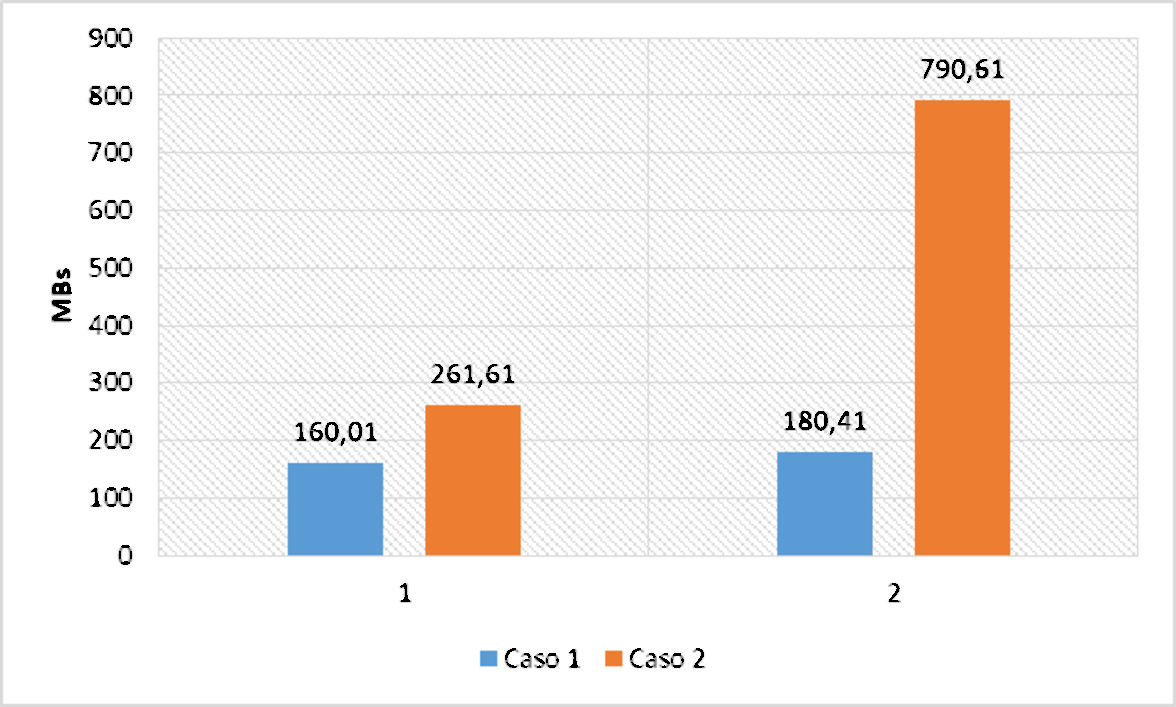
\includegraphics[scale=0.4]{imagenes/ram}
  \caption{Comparación consumo de RAM}
  \label{fig:ram}
\end{figure}

La figura \ref{fig:ram} evidencia la diferencia de consumo de RAM entre ambas opciones. Mientras que la primera apenas llega a los 200MBs, la segunda la cuadriplica. En consecuencia, será necesario contar con un PC de ciertas prestaciones para ser capaz de trabajar con redes grandes de usar este método.

\begin{figure}[H]
  \centering
  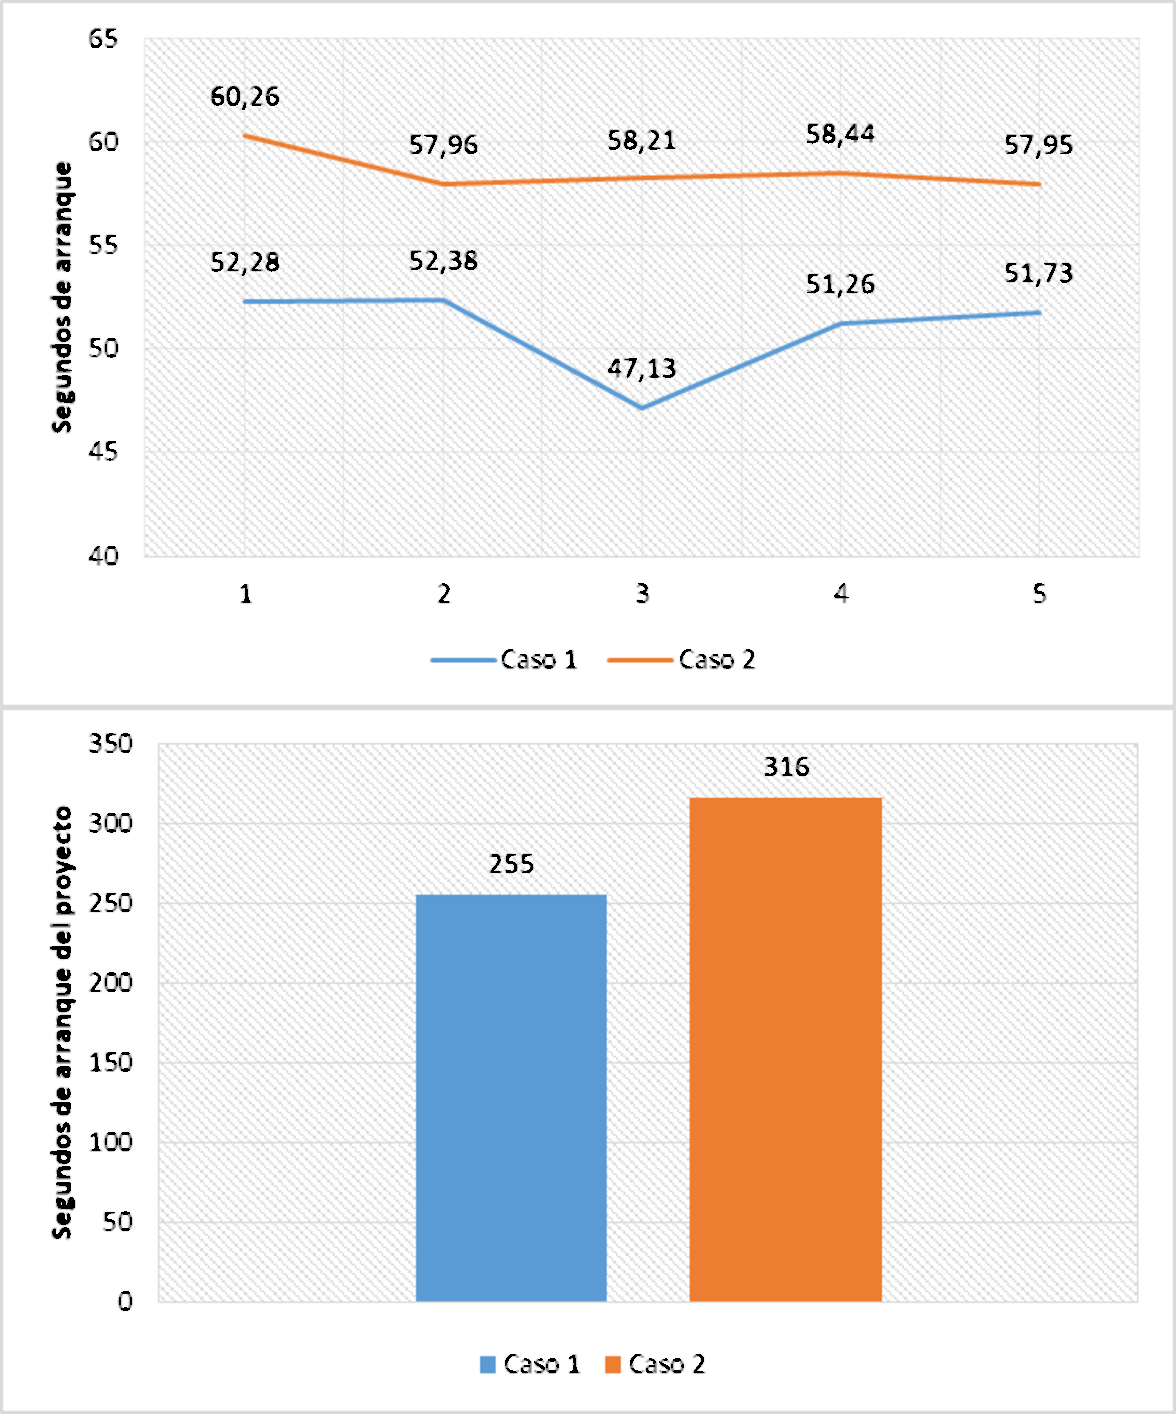
\includegraphics[scale=0.4]{imagenes/tiemposarranque}
  \caption{Tiempos de arranque de los nodos de forma individual (arriba) y en grupo (abajo)}
  \label{fig:tiemposarranque}
\end{figure}

El resultado también es negativo para el tiempo de arranque de los routers. Si bien en ninguno de los das casos la activación es automática como veníamos anunciando, el caso 2 sigue quedando detrás según se observa en la gráfica \ref{fig:tiemposarranque}. Es especialmente evidente en la activación grupal de estos, donde el tiempo de arranque del segundo caso es un 23,92\% mayor que el del primero.

\begin{figure}[H]
  \centering
  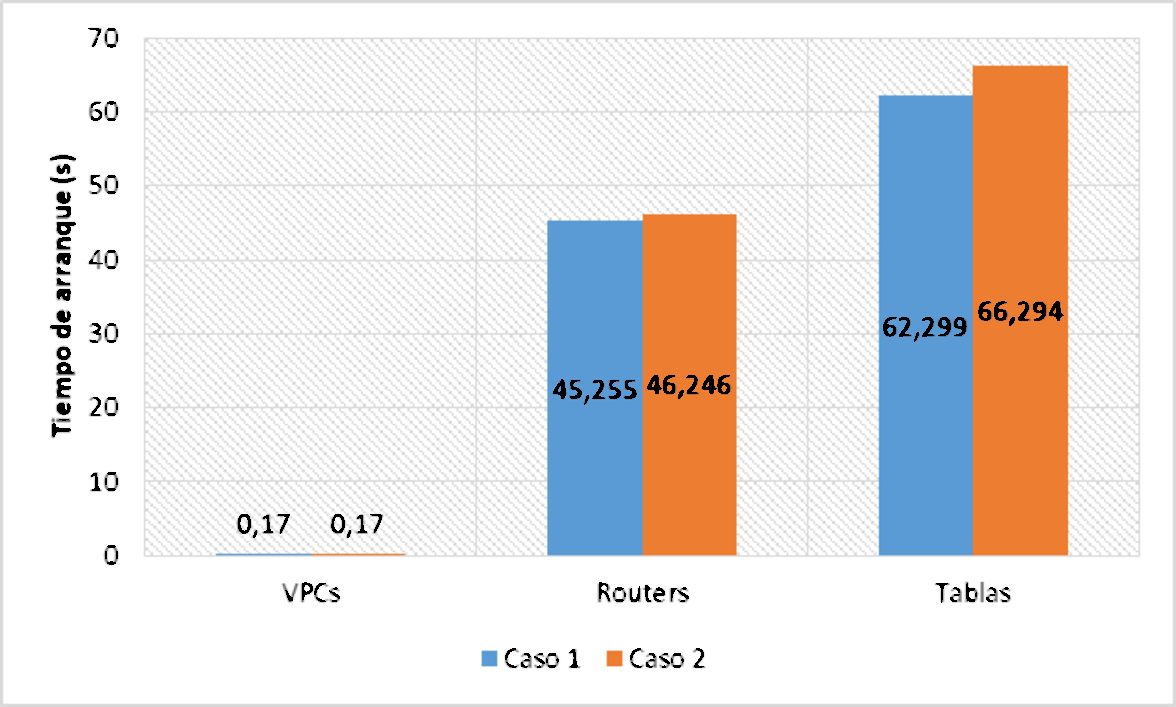
\includegraphics[scale=0.4]{imagenes/arranquejuego}
  \caption{Tiempos de arranque de las partes del juego relacionadas con el simulador}
  \label{fig:arranquejuego}
\end{figure}

Finalmente, la figura \ref{fig:arranquejuego} muestra que las diferencias a la hora de interactuar con el juego no son demasiado grandes entre los dos casos. El caso 1 es ligeramente más rápido que el segundo.

\section{Conclusiones}
El rendimiento del caso 2 es, en cada escenario, peor que el del caso 1. En las pruebas temporales la diferencia no es especialmente grande, de apenas unos segundos; quizá se evidencie más en el arranque grupal de los nodos, pero aún así no difieren más de 30 segundos. La principal problemática reside, como ha podido verse, en el consumo de memoria RAM, donde el primer caso supera con creces al segundo. 

Sin embargo, pese a este hándicap, sus ventajas son claras y fueron listadas al comienzo del capítulo. El hecho de aislar toda la configuración del simulador en una sola máquina virtual, hace su uso extremadamente portable y sencillo. Su principal problema, el consumo de RAM, no debe serlo a día de hoy, con sistemas que cuentan fácilmente con 8GBs de RAM. Además, la sola instalación de GNS3 es ya de por sí poco recomendable para equipos de pocas prestaciones \cite{gnsweb}. Yendo aún a más: si el proyecto se encuentra inicialmente activo y configurado cuando el juego se propone hacer uso de él, el caso 2 apenas se ve perjudicado frente al primero en cuanto a configuración del juego e interacción con este.

Consideramos entonces que es la opción correcta a seguir. Tratándose de un elemento que ha de ser compartido por los docentes hacia los alumnos, es importante para estos que ofrezca facilidad de instalación, la cual ofrece. Su portabilidad la convierte en la opción más interesante pese a los inconvenientes que es evidente que presenta.